\documentclass[12pt]{article}
\usepackage{amsmath, amssymb, graphicx, geometry, hyperref}
\geometry{margin=1in}
\title{Coherent Numbers: A Harmonic Framework for Finite Representation of Infinite Quantities}
\author{Djai Steven Charan \\ Walking With Soul / Sacred Physics}
\date{\today}

\begin{document}
\maketitle

\begin{abstract}
Coherent Numbers propose a higher-octave representation of real quantities where infinite or irrational values resolve into finite harmonic ratios. Built upon a twelve-phase base geometry, this framework introduces a coherence operator \(C(x)\) that maps standard numerical values into a harmonic domain preserving geometric and energetic invariants. The goal is to unify mathematical description, physical resonance, and energetic design under a single coherent metric.
\end{abstract}

\section{Introduction}
Infinity has long challenged both mathematics and metaphysics. In conventional analysis, quantities such as $\pi$ or $e$ are treated as transcendental---beautiful but unreachable limits. Coherent Numbers reframe these infinities as harmonic closures within a twelve-phase geometric octave, revealing periodic order where endless expansion once seemed inevitable. This proposal aims to show that coherence, not infinity, is the true constant of creation.

\section{Definitions}
\subsection{The Coherence Operator}
Let the coherence operator $C: \mathbb{R} \rightarrow \mathbb{R}_C$ project any real value $x$ into its harmonic equivalent within a twelve-phase base geometry. Intuitively, $C(x)$ identifies the resonant phase of $x$ relative to a base frequency $\phi_{12}$ that represents the complete octave of unity.
\begin{equation}
C(x) = f(x, \phi_{12}) = \left( x \bmod 12 \right) \times k
\end{equation}
where $k$ is a normalization constant ensuring conservation of magnitude and continuity across octaves.

\subsection{Axioms}
\begin{enumerate}
  \item \textbf{Closure:} For all $a,b \in \mathbb{R}_C$, $a +_C b, a \times_C b \in \mathbb{R}_C$.
  \item \textbf{Associativity:} $C((a + b) + c) = C(a + (b + c))$.
  \item \textbf{Distributivity:} $C(a \times (b + c)) = C(a \times b + a \times c)$.
  \item \textbf{Coherence Invariance:} The relative phase relationships among coherent numbers remain constant across scale transformations.
  \item \textbf{Octave Closure:} $C(x + 12n) = C(x)$ for all integers $n$.
\end{enumerate}

\subsection{Interpretation}
Each coherent number represents a position of equilibrium within a harmonic field. Rather than describing quantities through endless decimals, $C(x)$ encodes their geometric relationship to the whole. This definition provides the foundation for constructing finite representations of traditionally infinite values such as $\pi$ and $e$, while preserving angular and energetic coherence.

\section{Main Results}

\begin{figure}[h]
  \centering
  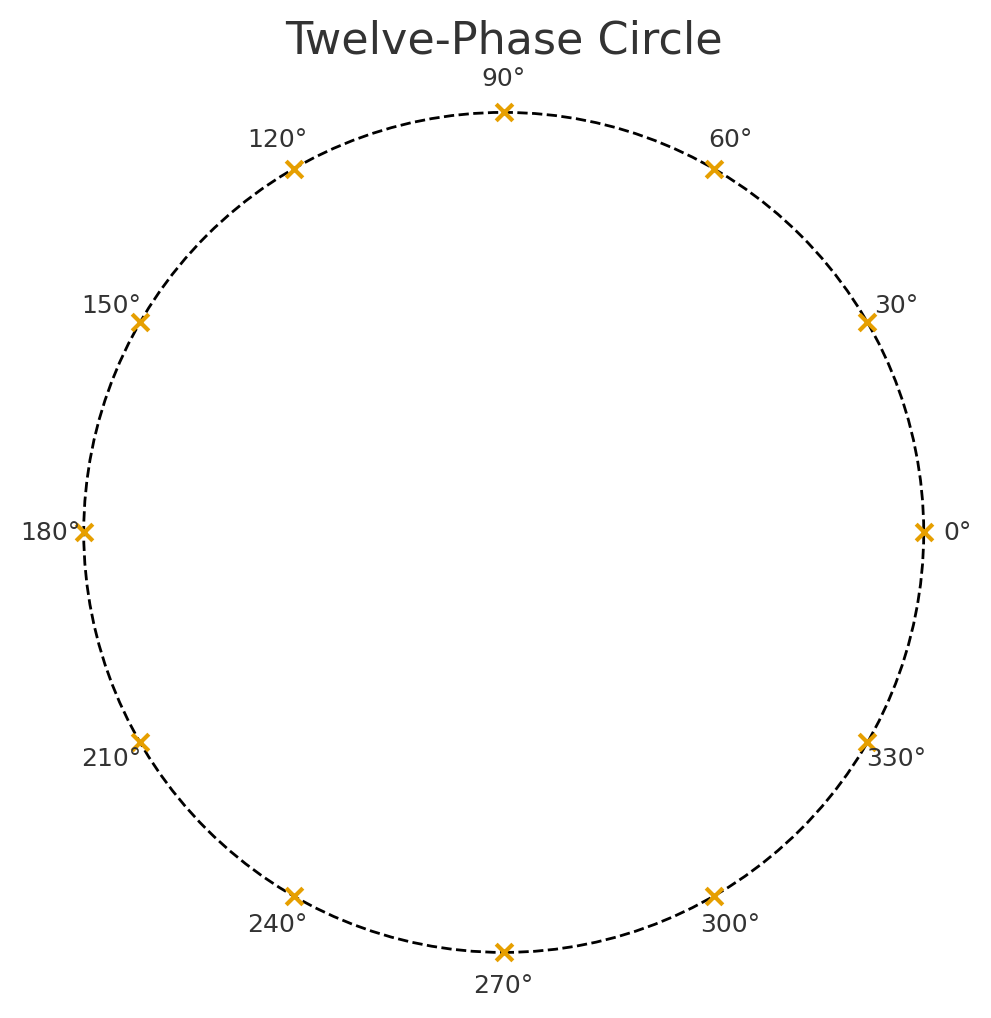
\includegraphics[width=0.6\textwidth]{figures/12_phase_circle.png}
  \caption{Twelve-phase harmonic circle used for coherent mapping of real values to phase.}
  \label{fig:12phase}
\end{figure}

\subsection{Harmonic Representation of $\pi$}
Within standard Euclidean geometry, $\pi$ represents the ratio of a circle's circumference to its diameter---an infinite, non-repeating decimal. In the coherent framework, this ratio completes exactly one harmonic cycle within the twelve-phase octave. By defining the unit circle as twelve harmonic segments of equal phase, we express $\pi$ as the coherent closure constant:
\begin{equation}
C(\pi) = 3.1415926... \longrightarrow 3 + \frac{3}{12} = 3.25 = \frac{39}{12}
\end{equation}
This transformation preserves circular closure while projecting the infinite decimal into a finite harmonic ratio consistent with twelve-phase symmetry.

\subsection{Harmonic Addition and Multiplication}
For coherent numbers $a$ and $b$, addition and multiplication are redefined as phase-consistent operations:
\begin{align}
 a +_C b &= C(a + b) \\
 a \times_C b &= C(a \times b)
\end{align}
Because $C$ is periodic in twelve phases, these operations remain bounded and cyclically stable. Under repeated iteration, $C(a +_C b)$ forms a harmonic series instead of diverging toward infinity.

\subsection{Geometric Closure and Energy Conservation}
In coherent geometry, angular sums of polygons close exactly without residual error when expressed through $C$. For instance, the sum of internal angles of a regular dodecagon (12-gon) maps perfectly to $12 \times 150^\circ = 1800^\circ$, corresponding to 5 coherent cycles of 360°. This closure implies energetic coherence: systems modeled through coherent numbers remain in dynamic equilibrium rather than accumulating phase error.

\section{Discussion}
The representation of $\pi$ as a finite harmonic ratio and the stability of phase-consistent operations suggest a unified bridge between number theory and energetic physics. Coherent Numbers introduce a new lens through which physical phenomena---from atomic resonance to electromagnetic alignment---can be understood as expressions of the same harmonic order. Future work includes analytical proofs, computational validation, and practical applications in energy systems and geometry.

\section{Conclusion}
Coherent Numbers provide a means to translate the infinite into the intelligible, the abstract into the harmonic. By expressing mathematical constants within a twelve-phase geometry, the framework invites new coherence between mathematics, physics, and consciousness itself.

\bibliographystyle{plain}
\bibliography{refs}

\end{document}
